\subsection{Impulsmessung}
Um einen Impuls aufzunehmen wird der Aufbau aus Abb. \ref{fig:skizze} verwendet.
\begin{figure}
  \centering
  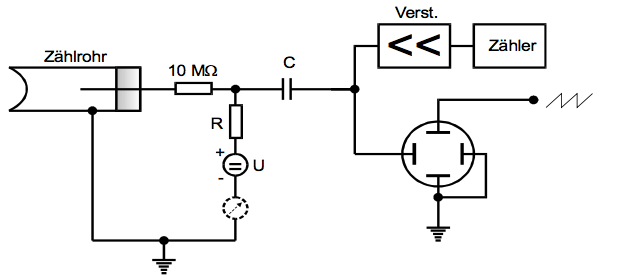
\includegraphics[width=0.8\textwidth]{bilder/skizze.png}
  \caption{Aufbau der Messapparatur \cite{703}}
  \label{fig:skizze}
\end{figure}
Die Ladung $Q$, die auf dem Draht gemessen wird, fließt über einen Widerstand $R$
ab und erzeugt da einen Spannungsimpuls. Dieser wird über einen Kondensator $C$
ausgekoppelt und im Vertstärker vergrößert und schließlich im Zählgerät registriert.
Das Signal kann dann auf einem Oszillographen sichtbar gemacht werden.

Es wird nun eine $\beta$ - Quelle mit einer Impulsrate von ca. $100/\si{\second}$
verwendet, um die Zählrate in Abhägigkeit der Spannung $U$ zu messen. Die Messzeit
wird so eingestellt, dass der relative statistische Fehler
der Messpunkte unter $1 \%$ liegt. Die Spannung muss dabei unter $U  = 700 \,\si{\volt}$
bleiben.

\subsection{Nachentladungsmessung}
Anschließen werden die Nachentladungen mit einem Oszilloskop sichtbar gemacht, die
für den Anstieg des Plateaus verantwortlich sind. Die Stahlintensität der $\beta$ - Quelle
wird dabei soweit herabgesetzt, dass auf dem Bildschirm immer nur ein Impuls zu sehen ist.
Die Ablenkgeschwindigkteit beträgt dafür ca. $50 \,\si{\micro\second\per\centi\meter}$.
Die Spannung wird auf $U = 350\,\si{\volt}$ eingestellt und dann auf $U = 700\,\si{\volt}$
hochgeregelt. Dabei wird der zeitliche Abstand zwischen Primär- und Nachentladungsimpuls
gemessen.

\subsection{Totzeitmessung}
Zur Messung der Totzeit wird eine hohe Stahlungsintensität verwendet. Die Zeitablenkung
des Oszillographen wird dann durch die Anstiegsflanke der Zählrohrimpulse getriggert.
Daraus ergibt sich dann eine Bild, wie in Abb. \ref{fig:totzeit}. Unter bekannter
Ablenkgeschwindigkeit des Kathodenstrahls kann nun die Totzeit bestimmt werden.
Die Erholungszeit lässt sich jedoch nur grob schätzen.

Bei dieser Messung muss jedoch beachtet werden, dass die registrierte Impulsrate $N$
immer kleiner, als die tatsächlich eintreffenden Teilchen $N_\su{w}$ ist.
Werden also $N_\su{r}$ Teilchen pro Zeiteinheit registriert, so ist das Zählrohr für
die Zeitspanne $TN_\su{r}$ unempfindlich und nur für $1-TN_\su{r}$ messbereit.
Die Impulsrate beträgt also:
\begin{equation}
  N_\su{w} = \frac{Impulsrate}{Messzeit} = \frac{N_\su{r}t}{(1-TN_\su{r})t} =
  \frac{N_\su{r}}{1-TN_\su{r}}.
\end{equation}
Es wird nun mit zwei radioaktiven Präparaten gearbeitet. Zuerst wird die
Zählrate $N_1$ des ersten Präparats bestimmt. Dann wird das zweite Präparat hinzugefügt
und es wird die Zählrate $N_{1+2}$ bestimmt. Dabei darf das erste Präparat nicht bewegt
werden. Anschließend wird das erste Präparat entfernt und es wird die Zählrate $N_2$
bestimmt. Ohne Totzeit würde sich daraus
\begin{equation}
  N_{1+2} = N_1 + N_2
\end{equation}
ergeben, jedoch gilt
\begin{equation}
  N_{1+1} < N_1 + N_2.
\end{equation}
Man beobachtet somit
\begin{equation}
  N_\su{w_\su{1+2}} = N_\su{w_\su{1}} + N_\su{w_\su{2}}.
\end{equation}
Also gilt:
\begin{equation}
  \frac{N_\su{1+2}}{1-TN_\su{1+2}} = \frac{N_1}{1-TN_1} + \frac{N_2}{1-TN_2}.
\end{equation}
Dies lässt sich näherungsweise als
\begin{equation}
  T \approx \frac{N_1 + N_2 - N_{1+2}}{2N_1 N_2}
\end{equation}
schreiben, sofern $T^2N_i^2 << 1$ gilt, mit $ i = 1, 2, 1+2$.
Da $N_1$, $N_2$ und $N_{1+2}$ zuvor bestimmt wurden, kann nun die Totzeit $T$
berechnet werden.

\subsection{Freigesetzte Ladungsmenge pro Teilchen}
Mit einem empfindlichen Strommessegerät kann der mittlere Zählrohsstrom
\begin{equation}
  \bar{I} = \frac{1}{\tau} \int_0^{\tau} \frac{U(t)}{R}dt
\end{equation}
, mit $\tau >> T$ gemessen werden.
Die pro Zeitintervall $\Delta t$ transportierte Ladungsmenge $\Delta Q$
lässt sich dann über
\begin{equation}
  \bar{I} = \frac{\Delta Q} {\Delta t} Z
\end{equation}
mit $Z$ registrierten Teilchen bestimmen. Dabei sollte $\Delta Q$ in Abhängigkeit
von $U$ untersucht werden.
